\section{Results}\label{sec:results}

\subsection{Sigma Hyperparameter Selection}\label{subsec:sigmaHyperparameterSelectionResults}
Recall that $\sigma_1, \sigma_2, \ldots \sigma_n$ are hyperparameters that must be defined prior to executing the
algorithm.
The grid search exhausts every permutation $P_n^{\sigma_n}$, where:
\begin{equation}
    \label{eq:gridSearchQuerySigma}
    \sigma_n \ \in \ \{10^{-16}, 10^{-15}, \ldots 10^{1}\}
\end{equation}
% 2.22 * 10^-16 is the machine epsilon for double

\begin{figure*}
    \centering{
    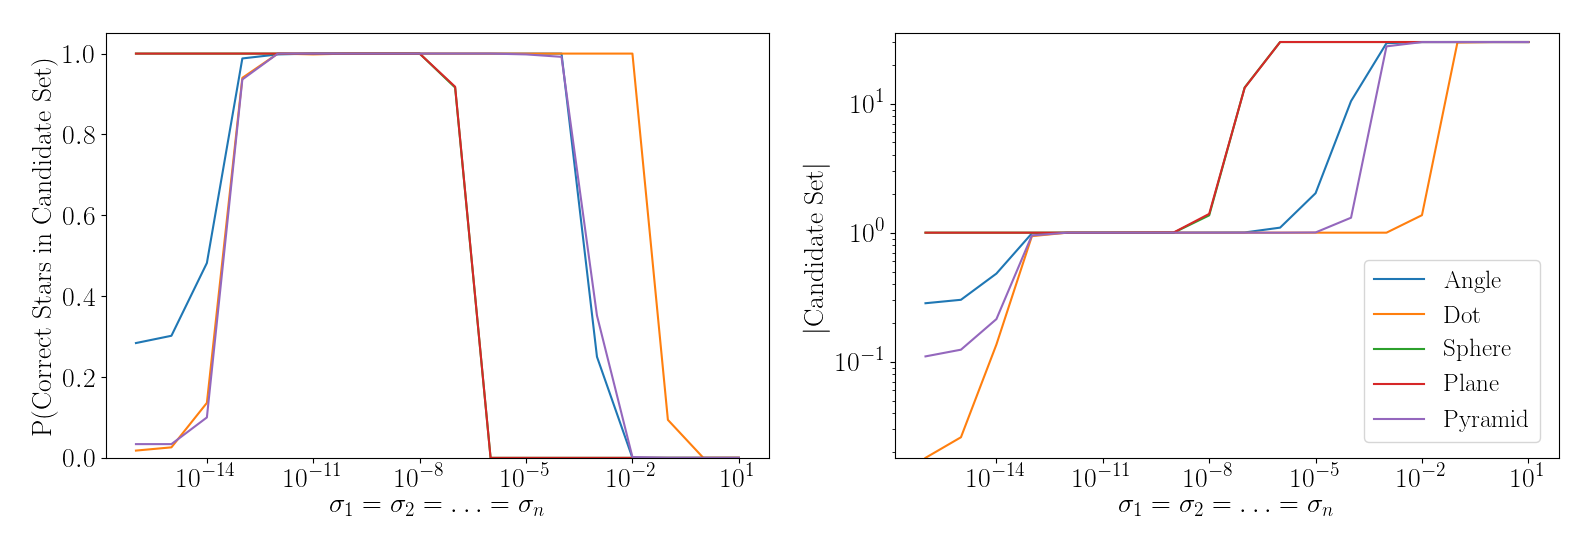
\includegraphics[scale=0.45]{images/sigma1-pcss-css.png}
    \caption{
    The left plot depicts the effect of varying $\sigma$ on the probability that the correct star set exists in the
    resulting candidates after the query.
    The right plot depicts the effect of varying $\sigma$ on the average size of the candidate set after the query, bounded
    by 30 candidates at maximum.
    The field-of-view is bounded by $f = 20^\circ$ and the apparent magnitude is bounded by $m = 6.0$.
    Each point represents the average of 1000 query steps without noise introduced.
    For brevity, all deviations associated with methods of more than one feature term (i.e.\ Dot Angle, Spherical
    Triangle, \ldots) had all corresponding $\sigma$ terms set equal to each other.
    } \label{figure:sigmaHyperparameterPlots}
    }
\end{figure*}

The set of plots in~\autoref{figure:sigmaHyperparameterPlots} depict the effect on different $\sigma$ terms against the
average size of the candidate set $S$ (on the left) and the probability that the correct stars exist in this candidate
set $Q$ (on the right).
If the deviation is too small, then the selectivity of each query becomes too restrictive and no results are returned.
On the other hand when the selectivity is too high, the candidate set size upper bound of 30 candidates is
hit and the chance that the correct candidate exists in the query declines.

The ideal period for all methods identifying images restricted by $f < 20 \land m < 6.0$ occurs when:
\begin{equation}
    \label{eq:idealRegionAcrossFeatures}
    \sigma_n \ \in (10^{-12}, 10^{-8})
\end{equation}
Regardless of the feature, a deviation choice between these bounds should be acceptable for distinguishing stars.

% Not including this, don't feel it is relevant to ideal analysis.
%It is important to note that each feature exists in different bounds.
%The values below represent the observed bounds of each feature:
%\begin{alignat*}{2}
%    \label{eq:observedFeatureSpace}
%    % Non-inclusive bounds given below.
%    \theta^{ij} &\in (2.6 \times 10^{-3} &&, 2.0 \times 10^1) \\
%    \theta^{ij} &\in  (2.6 \times 10^{-3} &&, 2.0 \times 10^1) \\
%    \theta^{ic}, \theta^{jc} &\in (2.6 \times 10^{-3} &&, 2.0 \times 10^1) \\
%    \phi &\in (1.3 \times 10^{-3} &&, 1.8 \times 10^2) \\
%    a^{ijk} &\in (3.1 \times 10^{-9} &&, 5.4 \times 10^{-2}) \\
%    \imath^{ijk} &\in (4.8 \times 10^{-16} &&, 5.3 \times 10^{-4}) \\
%    a^{ijk} &\in (3.7 \times 10^{-9} &&, 5.3 \times 10^{-2}) \\
%    \imath^{ijk} &\in (4.9 \times 10^{-16} &&, 5.3 \times 10^{-4})
%\end{alignat*}

% TODO: Replace these values with the ones using the most recent dataset.
\begin{table}
    \centering {
    \caption{
    Ideal query hyperparameter determination and sensitivity results of each method.
    The ideal region length $\ell$ represents the number of deviations where~\autoref{eq:idealQuery} is held.
    Each method's critical points $\sigma_{c1}$ and $\sigma_{c2}$ a is the upper bound on the $Q$ and $S$
    ideal region.
    } \label{tab:sensitivityIdealResults}
    \begin{tabular}{m{0.27\columnwidth}|m{0.13\columnwidth}|m{0.2\columnwidth}|m{0.2\columnwidth}}
        \textbf{Method} & $\ell$ & $\frac{\partial Q}{\partial\sigma} \text{ at } \sigma_{c1}$ &
        $\frac{\partial S}{\partial \sigma} \text{ at } \sigma_{c2}$ \\
        \hline \hline
        \textbf{Angle} & 3 & -0.375 & 0.001 \\ \hline
        \textbf{Dot Angle} & 9 & -0.453 & 0.183 \\ \hline
        \textbf{Spherical \newline Triangle} & 8 & -0.042 & 0.181\\ \hline
        \textbf{Planar \newline Triangle} & 6 & -0.041 & 0.001 \\ \hline
        \textbf{Pyramid} & 7 & -0.001 & 0.002
    \end{tabular}
    }
\end{table}

Referencing~\autoref{tab:sensitivityIdealResults}, there appears to some correlation between the number of
\textit{distinct} features and length of the stability region here.
The Dot Angle method uses three total features, two of which are distinct from each other ($\theta$ vs. $\phi$) for
it's query.
The Pyramid method uses three similar features, which has the same stable region length as the triangle methods
using two distinct features.
The Angle method uses only one feature for its query, and suffers in stable region length.

The candidate set size responses are most likely a result of the size of possible candidates that belong to each
method's respective feature (i.e.\ the number of rows of the table used in query).
The Angle method has the least number of possible candidates given the $f < 20 \land m < 6.0$ constraint, at 353700
possible catalog sets.
The triangle methods have roughly 35 times as many possible catalog sets as the Angle method.
The Dot Angle method has 3 times as many possible catalog sets as the triangle methods, and roughly 105 times as many
possible catalog sets as the Angle method.
Given a larger pool of results to choose from, it follows that the number of false positive increases as well.

The largest $Q$ response belongs to the Dot Angle method, while the smallest response belongs to the Pyramid method.
Unlike the candidate set size response, there appears to be no obvious correlation between the response of correct
star set existence and the number of features used.
If noise is not known, the most forgiving feature set in terms of both responses is the Pyramid method.

The $\sigma$ parameters for the following experiments were chosen using the results of the grid search.
The largest $\sigma_1, \sigma_2, \sigma_3$ (ordered as such) that maintained all the conditions in~\autoref{eq:idealQuery} and whose
parameters did not exceed the ideal region are described below.
\begin{alignat*}{2}
    \text{Angle}&: \sigma_\theta &&= 10^{-4}\\
    \text{Pyramid}&: \sigma_\theta &&= 1.0 \times 10^{-4}\\
    \text{Dot Angle}&: \sigma_{\theta_{ic}} &&= 10^{-2}, \sigma_{\theta_{jc}} = 10^{-2}, \phi = 10^{-2} \\
    \text{Spherical Triangle}&: \sigma_a &&= 10^{-9}, \sigma_\imath = 10^{-9} \\
    \text{Planar Triangle}&: \sigma_a &&= 10^{-9}, \sigma_\imath = 10^{-9}
\end{alignat*}

In addition to the $\sigma_n$ parameters used in the previous experiments, a parameter $\sigma_o$ must be defined
prior to executing the \Call{FPO}{} method.
The linear search exhausts every overlay deviation selection:
\begin{equation}
    \label{eq:linearSearchSigmaOverlay}
    \sigma_n \ \in (10^{-16}, 10^{2})
\end{equation}

\begin{figure*}
    \centering{
    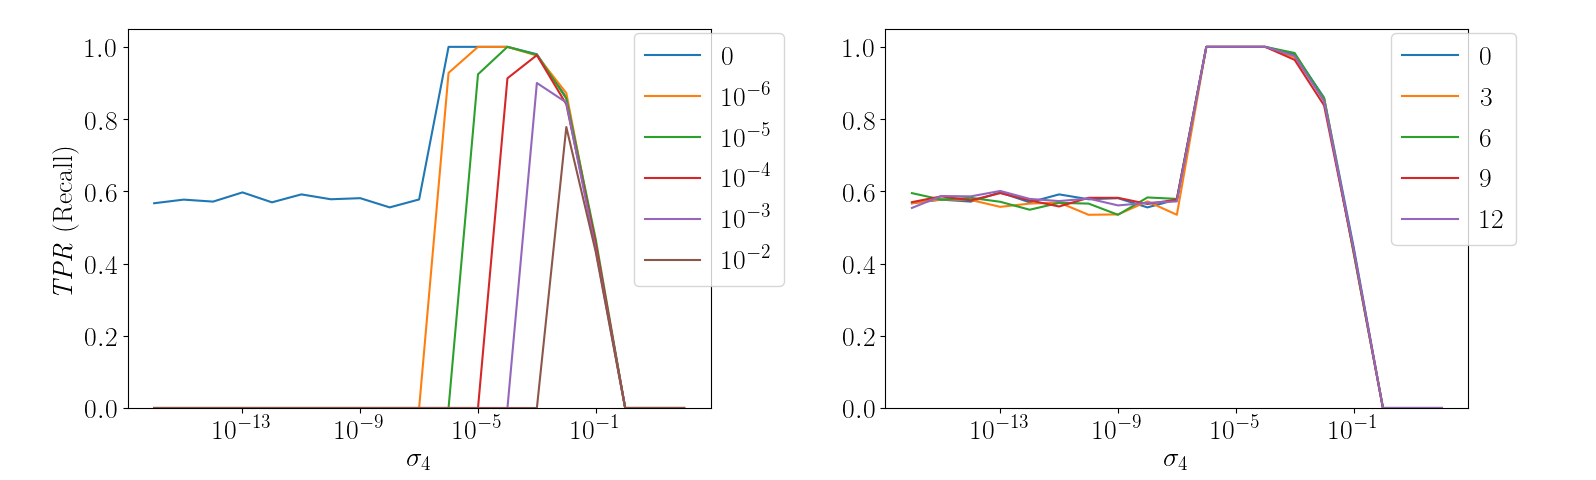
\includegraphics[scale=0.45]{images/sigma4-recall.png}
    \caption{
    Both plots depict the effect of varying $\sigma$ on the recall.
    The left plot depicts this relationship for different variations in noise, while the right plot depicts the same
    relationship for different numbers of false stars.
    The field-of-view is bounded by $f = 20^\circ$ and the apparent magnitude is bounded by $m = 6.0$.
    Each point represents the average of 200 query steps.
    } \label{figure:sigmaOverlayHyperparameterPlots}
    }
\end{figure*}

The set of plots in~\autoref{figure:sigmaOverlayHyperparameterPlots} depict the effect on different $\sigma$ terms
against the recall.
The period of accurate stability for Gaussian noise under $\sigma = 10^{-5}$ and for all false star introductions occurs
when:
\begin{equation}
    \label{eq:sigmaOverlayStableRegion}
    \sigma_4 \ \in (10^{-6}, 10^{-3})
\end{equation}

Looking at the both plots it is interesting to note that under no noise (Gaussian or false stars), a $\sigma_4 \ \in
(10^{-17}, 10^{-6})$ gives a recall of $~0.57 \pm 1.8 \times 10^{-2}$.
This suggests that a slightly noisier image \textit{might} give more accurate \Call{DMT}{} results, but the use of
additional filters should normalize these results.
On the other end of the stability period for $\sigma_4 > 10^0$, accuracy drops straight to 0 regardless of the noise
presented.
At this period, the \Call{DMT}{} procedure would likely find any configuration given as not confident.

Focusing on the left plot of varying Gaussian noise, the accuracy dips to zero once the deviation of Gaussian noise
exceeds the selected deviation.
Past the $10^{-4}$ mark, the largest accuracy a deviation choice can achieve is no longer equal to one.
If noise is known, then the appropriate deviation for the \Call{FPO}{} method can be selected.
The right plot shows that the accuracy is not affected under different amounts of false stars.
Given varying amounts of false stars, virtually none of these stars were identified as an actual star.
The \Call{FPO}{} method is seen as highly specific, yielding no false positives.

The value of $\sigma_4 = 10^{-4}$ was selected for use in the \Call{FPO}{} method.
This is the largest deviation that lies in the accurate stable region.

\subsection{Query Selectivity}\label{subsec:querySelectivityResults}
Using the optimal hyperparameters described in the previous section, each query step was analyzed in terms of its
$Q$ and $S$ response to an introduction of Gaussian noise.

\begin{table}
    \centering {
    \caption{
    Each method's probability that the correct star set exists after querying ($Q$), average candidate set size ($S$),
    and query running time $t$ under no noise.
    Each point represents the average of 1000 query steps.
    } \label{tab:queryExperimentResults}
    \begin{tabular}{m{0.18\columnwidth}|m{0.2\columnwidth}|m{0.2\columnwidth}|m{0.2\columnwidth}}
        \textbf{Method} & $Q$ & $S$ & $t \ (ms)$  \\
        \hline \hline
        \textbf{Angle} & 1.00 & 10.68 & 150.76 \\ \hline
        \textbf{Dot Angle} & 1.00 & 1.38 & 192.48 \\ \hline
        \textbf{Planar \newline Triangle} & 1.00 & 1.01 & 152.44 \\ \hline
        \textbf{Spherical \newline Triangle} & 1.00 & 1.01 & 152.48\\ \hline
        \textbf{Pyramid} & 0.99 & 1.33 & 165.71
    \end{tabular}
    }
\end{table}

In~\autoref{tab:queryExperimentResults}, each method's $Q, S, \text{ and } t$ is displayed without the presence of
noise.
Given that no noise is included, it is expected that all methods have 100\% accuracy- but the Pyramid method contains
6 points out of 1000 where the correct image subset does not exist after querying.
The most likely source of error here are steps 6, 7, 8 in~\autoref{algorithm:pyramidIdentification} to produce the
$T$ sets.
A trade off of space (i.e.\ a larger catalog of precomputed trios) would avoid the common stars routine at runtime,
which would reduce these steps to one and potentially increase accuracy.

The Pyramid and Angle method use the same catalog, which is $\sim$35 times as small as the triangle method's catalog.
The Angle method also involves only one image feature filter ($\theta$) to obtain the desired result, in comparison
to the two image feature filters ($a, i$) of the triangle methods.
Querying a small catalog with a single filter allows the Angle method to achieve the fastest query step of 150.8ms.
Trailing closely by an average of 1.7ms are the Spherical and Planar Triangle methods.

Even though the Pyramid method uses the same catalog as the Angle method and only requires a single image feature
filter ($\theta$), it must perform three separate catalog accesses and find the common stars.
Consequently, in fourth place is the Pyramid method.
This method runs 13.3ms slower than the triangle average.
The Dot Angle catalog is 3 times as large as the triangle catalogs, or $\sim$105 times larger than the Angle and Pyramid
catalogs.
This query also involves three image feature filters ($\theta_1, \theta_2, \phi$) to obtain the desired result, and
as a result runs 1.28 times slower than the fastest query step (Angle method).

In terms of candidate set size, the triangle methods consistently produce the smallest average candidate set
(combined average of 1.01 sets).
For all 1000 runs, there were only 6 points for the Planar Triangle method and 5 points for the Spherical Triangle
method where the candidate set size where~\autoref{eq:nonUniqueCandidateSet} holds.
If the condition below is not true, then the reduction step can essentially be skipped (leading to faster end-to-end
runtimes).
\begin{equation}\label{eq:nonUniqueCandidateSet}
    |R| \neq 1
\end{equation}
For these 6 points of the Planar Triangle method, the average candidate set size was 2.00 sets.
For these 5 points of the Spherical Triangle method, the average candidate set size is 2.20 sets.
Given no noise, the planar triangle features are more distinctive than the spherical triangle features.

Third place in candidate set size is the Pyramid method, which had 243 / 1000 points
where~\autoref{eq:nonUniqueCandidateSet}.
The average candidate set size for these 243 points is 1.33 sets.
In fourth place is the Dot Angle method, having 294 points of average candidate set = 2.28 sets for all points where
~\autoref{eq:nonUniqueCandidateSet}.

In last place by a large margin is the Angle method, which is a factor of 10.61 sets larger than the triangle method.
For all 1000 points, 979 of these did not have a candidate set size equal to 1.
The Angle method has the fastest query time, but the sole image feature $\theta$ is not unique enough to identify one
star pair.

Using the measure for efficiency in~\autoref{eq:queryEfficiency}, each method ranks as follows:
\begin{multicols}{2}
    \begin{enumerate}
        \item Planar Triangle
        \item Spherical Triangle
        \item Pyramid
        \item Dot Angle
        \item Angle
    \end{enumerate}
\end{multicols}

Both the Spherical and Planar Triangle methods have the most efficient query step.

\subsection{Candidate Reduction}\label{subsec:candidateReductionResults}
Using the same optimal hyperparameters described in~\autoref{subsec:sigmaHyperparameterSelectionResults}, each query +
reduction step was analyzed in terms of the average accuracy and efficiency response to Gaussian noise and false stars.

\begin{figure*}
    \centering{
    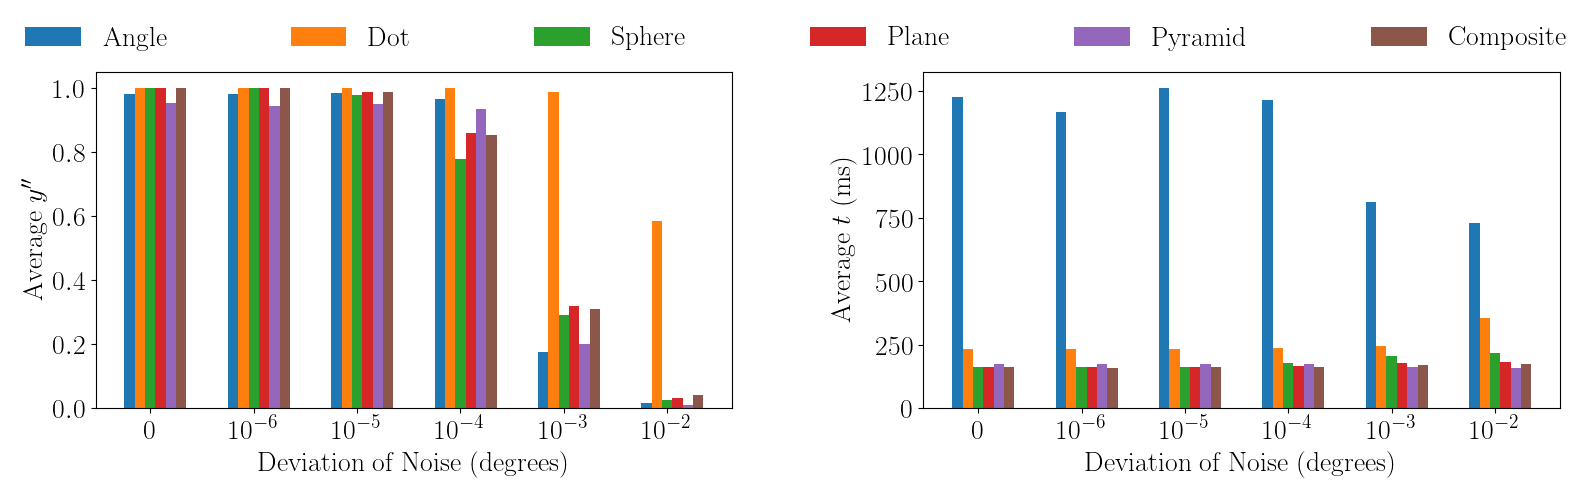
\includegraphics[scale=0.45]{images/reduction-shift-exp.png}
    \caption{
    Both plots depict the effect of varying the deviation of Gaussian noise on the average accuracy (left) and
    average running time to produce an $r$ set (right) for different identification methods.
    The field-of-view is bounded by $f = 20^\circ$ and the apparent magnitude is bounded by $m = 6.0$.
    Each method was capped at 500 query steps before erroring out and producing a false result.
    Each point represents the average of 1000 reduction steps.
    } \label{figure:reductionShift}
    }
\end{figure*}

Without noise in both~\autoref{figure:reductionShift} and~\autoref{figure:reductionFalse}, only the Angle method
(98.4\%) and Pyramid method (95.5\%) do not have 100\% accuracy in reduction.
The Angle method has the fastest query step, but is heavily slowed down by its $\{ R \mid 1 = |R|\}$ reduction step.
In the no noise case the Angle method is shown to have the correct candidates at query time for all runs- but
the large candidate set size at query time coupled with the single candidate set filter leads to more query-reduction
looping.
The Angle method accessed the catalog 46.2 more times and runs 6.86 longer than the other identification methods on
average.
The longest recorded time for the no noise image case is 7554.0ms from this method.
For all 1000 points in the no noise case, there only exist 17 points where a sole candidate result is returned for the
first query.

The slight inaccuracies of the Pyramid method under no noise are magnified at reduction time, now dipping 3.8\% below
its query time accuracy and ranking.
This method consumes 3.00 catalog accesses on average to obtain an answer, which is the amount of accesses required
for a single Pyramid query.
This suggests that the $\{ R \mid 1 = |R|\}$ filter may not be restrictive enough for this method.
Rather than aggressively verify here, the Pyramid method would rather pass the candidate set to its verification routine
\Call{VerifyP}{} at the identification step.
Consequently, the reduction accuracy dips here.

The Dot Angle method is the next slight outlier, which also uses the $\{ R \mid 1 = |R| \}$ reduction step.
Again, the aggressiveness of the single candidate set filter is observed here.
There exists 720 / 1000 points where a single candidate set was returned after the first query, meaning the remaining
280 had to perform additional queries.
28\% of the time though, this process consumed on average 2.58 catalog queries to meet the single candidate set
requirement.

Ranked 4th in running time is the Pyramid method, with an average query step count and running time of 1.00 steps
($\sim$3.00 catalog accesses) and 231.0ms respectively.
The reduction step is the same as the Dot Angle and Angle method.
There exists only 1 / 1000 points where~\autoref{eq:nonUniqueCandidateSet} holds, having
There are slightly more cases where the query step only has to be performed once in comparison to the Dot Angle method,
but these differences magnify the flaw of the expensive Dot Angle query step.

In 1st, 2nd, and 3rd place are the Planar Triangle method, Composite Pyramid method, and Spherical Triangle method
respectively.
All of these methods have an average runtime of $159.2 \pm 24.7$ms, consuming 1 query set on average to obtain a result.
The Spherical and Planar Triangle methods use the \Call{Pivot}{} reduction step, but the majority of the $R$ reducing
comes from their efficient query steps.
For all methods combined (total of 3000 points), there exist only 12 reduction runs
where~\autoref{eq:nonUniqueCandidateSet} applied.
Of these 12, only one additional query was required to reduce the candidate sets to a sole element.

In~\autoref{figure:reductionShift}, the deviation of Gaussian noise against the average accuracy and runtime is
displayed for different identification methods.
As soon as Gaussian noise of $10^{-5}$ degrees is introduced, all methods using triangular features can no longer
promise 100\% accuracy (average of 1.5\% decrease).
The Pyramid and Angle methods experience an average decline in accuracy of 76.3\% with Gaussian noise of $10^{-3}$
degrees from $10^{-4}$ degrees.
The Dot Angle method, with the largest query $\sigma$ parameter experiences a decline of 40.3\% with noise of $10^{-2}$
degrees from $10^{-3}$ degrees.

Note that the hyperparameters for all methods were chosen without any noise introduced.
The upper bound of the ideal region for the angular separation feature (Angle and Pyramid) was $\sigma_1 = 10^{-4}$.
The upper bound of the ideal region for the Dot Angle features was $\sigma_{(1, 2, 3)} = 10^{-2}$.
It follows that any angular noise greater than this should lead to a decline in accuracy.

For methods using triangular features, the answer is not as easy to determine.
The Planar Triangle, Spherical Triangle, and Composite Pyramid method's accuracy decreases to an average of
83.0\% for noise of $10^{-4}$ degrees.
At $10^{-3}$, all triangular methods decreases to 30.7\%.
Beyond this, accuracy drops very close to zero (3.2\% at $10^{-2}$ degrees).
The triangle methods would be less sensitive to noise if the $\sigma$ parameters were increased, but this comes at the
price of time.
This can be observed with the Dot Angle method who is able to promise near-to 100\% accuracy longer than all other
methods, but does run slightly slower than every procedure except for the Angle method.

Looking at the running time plot on the right, all methods except for the Angle and Dot Angle methods are fairly
consistent as noise is increased.
Intuitively, larger noise should lead to longer reduction times.
Each method's reduction step would have to iterate through more stars in the image to find the subset that fits the
reduction criteria.
The Angle method though, does not follow this reasoning.
This method actually decreases in time as $10^{-3}$ degrees of noise is introduced from $10^{-4}$ degrees, running
400.2ms faster and consuming 25.1 less query steps.
The fact that the Angle method is taking faster to run and using less catalog accesses under more noise suggests that
the method arrives at false answers quicker than accurate ones.
Once noise goes beyond the $\sigma_1$ query parameter, the correct pair found less noisy images no longer meets the
query criteria.

As $10^{-4}$ degrees of noise is introduced, all methods using triangular features run 6.4ms longer on average.
The average query step count increase from $10^{-5}$ degrees of noise to $10^{-4}$ degrees is 46.2 steps (6.87 steps vs.
51.5 steps).
Increasing the noise to $10^{-3}$ degrees, these same methods run 14.9ms longer.
The average query step count increases by a factor of 3.6 here, or 134.5 steps.
Both the $\{ R \mid 1 = |R| \}$ and pivoting reduction step generally handle this type of noise the same.
As the noise increases with these methods, so does the number of catalog accesses and the running time.

The Dot Angle method experiences the largest jump in runtime as noise increases from $10^{-3}$ degrees to $10^{-2}$.
Runtime increases 110.9ms, and the average number of catalog accesses increases by 1.73.
For noise beyond the $\sigma_{(1, 2, 3)}$ parameters, the aggressiveness of the $\{ R \mid 1 = |R| \}$ reduction step
is seen as more iterations are required to obtain an accurate result or error out.

The Pyramid method has the most consistent running time of all methods here, running an average of
$166.1 \pm 6.5$ms for all of the trials associated with this type of noise.

\begin{figure*}
    \centering{
    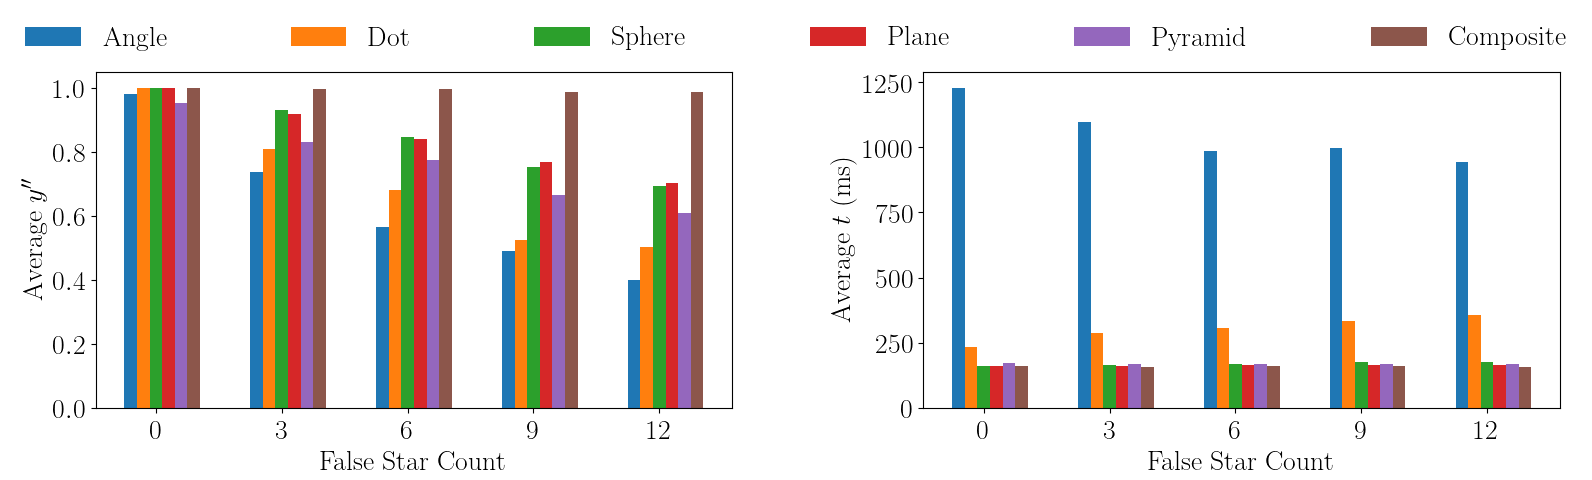
\includegraphics[scale=0.45]{images/reduction-false-exp.png}
    \caption{
    Both plots depict the effect of varying the number of false stars on the average accuracy (left) and
    average runtime to produce an $r$ set (right) for different identification methods.
    The field-of-view is bounded by $f = 20^\circ$ and the apparent magnitude is bounded by $m = 6.0$.
    Each method was capped at 500 query steps before erroring out and producing a false result.
    Each point represents the average of 1000 reduction steps.
    } \label{figure:reductionFalse}
    }
\end{figure*}

In~\autoref{figure:reductionFalse}, the number of false stars against the average accuracy and runtime is displayed
for different identification methods.
Here, all methods except for the Composite Pyramid method experience a negative accuracy response to this noise.
The list below orders each method from least responsive to most responsive from 0 to 12 false stars.
\begin{multicols}{2}
    \begin{enumerate}
        \item Composite Pyramid
        \item Planar Triangle
        \item Spherical Triangle
        \item Pyramid
        \item Angle
        \item Dot Angle
    \end{enumerate}
\end{multicols}

The Angle and Dot Angle methods experience the largest decline from no noise to 12 false stars of 58.6\% and 49.7\%
respectively.
Both methods specify no protection against this type of noise beyond the features themselves, and it follows that
both of these rank last in terms of false star tolerance.
In both~\autoref{algorithm:angleIdentification} and~\autoref{algorithm:dotAngleIdentification}, combinations are chosen
using nested loops.
An example sequence of trios (i.e.\ the three nested loop case) is depicted in~\autoref{eq:simple3NestedLoop} for
$n = 5$ stars.
\begin{equation}\label{eq:simple3NestedLoop}
a_{simple} = ( \{1,2,3\}, \{1,2,4\}, \{1,2,5\}, \{1,3,2\}, \ldots )
\end{equation}

If a false star exists in the outermost loop to produce trios, then each following $n^2$ combination will be incorrect
until the star in the outer loop changes.
This gives the Dot Angle method $n^2$ more opportunities to choose a wrong trio in this case, and is likely why it is
the most responsive to false stars.
The Angle method method only requires two nested loops, which gives only $n$ incorrect combinations if a false star
exists in the outer loop.
This higher turnover allows the Angle method to perform only slightly worse than the rest of the methods (besides
the Composite Pyramid).

The Spherical and Planar Triangle methods use the same method to choose combinations as the Dot Angle method, but differ
in their use of the \Call{Pivot}{} method and their query features.
If a false star is chosen in the outer loop for either of the triangle methods, the addition of the \Call{Pivot}{} call
gives $n^2 \times n = n^3$ more opportunities to choose the wrong trio.
Even though this is a factor of $n$ worse than the Dot Angle method, the efficiency of the query step for these
methods appear to mitigate the potential errors.

Both the Composite Pyramid and Pyramid methods specify a false star persistence avoidance process for choosing
query star sets as opposed to the simple triple nested loops of the other methods.
An example sequence of this process given an image of $n=5$ stars is depicted below.
\begin{equation}\label{eq:pyramidNestedLoop}
a_{pyramid} = ( \{1,2,3\}, \{2,3,4\}, \{3,4,5\}, \{1,2,4\}, \ldots)
\end{equation}
If star 1 was a false star in~\autoref{eq:pyramidNestedLoop}, then the next element would not use it.
This works well in increasing the accuracy of the Composite Pyramid method's reduction step, but not in the Pyramid's
reduction step.
This is likely due to the Pyramid method's weak reduction step, which does not allow for high turnover.
The avoidance process will not wok in the Pyramid method's favor if it does not choose new query sets.

The running time plot again shows that the Angle method runs faster when more noise is introduced.
From 0 to 12 false stars, the Angle method runs 269.7ms faster and consumes 18.0 less query steps on average.
Incorrect answers fit the reduction criteria better than correct ones here.
From 0 to 12 false stars, the Pyramid method performs 1.2 more query steps (3.8 catalog accesses) on average.
Similarly, the Composite Pyramid method only accesses the catalog 2.8 more times on average.

The Planar and Spherical Triangle methods both exhibit slight runtime response to an increasing number of false
stars.
From 0 to 12 false stars, the Planar Triangle method increases in runtime by 5.6ms and consumes 84.0 more catalog
accesses on average.
The Spherical Triangle method increases in runtime by 18.9ms, but only consumes 73.0 more query sets on average.

Second to last in both runtime and accuracy given false stars is the Dot Angle method.
Recall that this was the most accurate under the largest amount of noise, but the slowest of the six.
From 0 to 12 false stars, the Dot Angle method increases in runtime by MP79ms and accesses the catalog MP80 more times
on average.
On average, a 3 false star increase leads to $MP81 \pm SP4$ms increase in running time and $MP82 \pm SP5$ more
catalog accesses.

For the most accurate reduction step given Gaussian noise given the selected hyperparameters, the Dot Angle method
performs the best.
If a faster variant is desired against the same type of noise, the Pyramid method's accuracy is slightly worse but
is more consistent and faster.
When dealing with false stars, the most consistently fast and accurate reduction step belongs to the Composite Pyramid
method.

\subsection{Identification Determination}\label{subsec:identificationDeterminationResults}
Using all optimal hyperparameters described in~\autoref{subsec:sigmaHyperparameterSelectionResults}, each identification
was ran end-to-end and analyzed in terms of its response to an introduction of Gaussian noise and false stars.
The number of catalog accesses

\begin{figure*}
    \centering{
    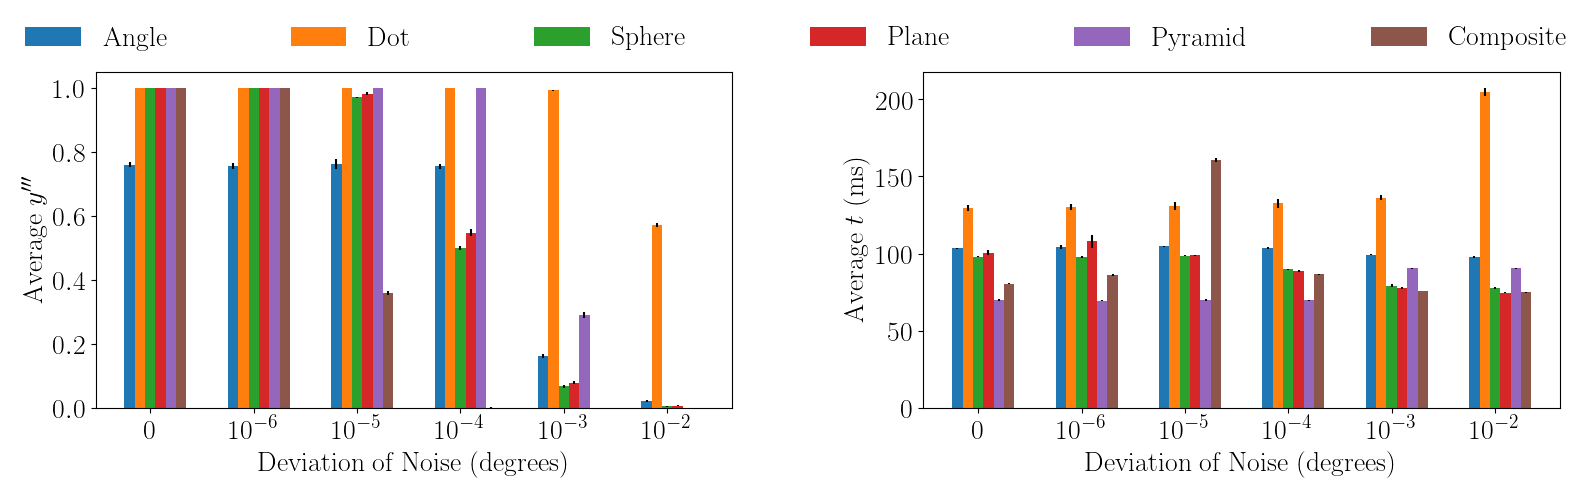
\includegraphics[scale=0.45]{images/identification-shift-exp.png}
    \caption{
    Both plots depict the effect of varying the deviation of noise on the average accuracy (left) and average
    running time to produce a map $a$ (right) for different identification methods.
    The field-of-view is bounded by $f = 20^\circ$ and the apparent magnitude is bounded by $m = 6.0$.
    Each method was capped at 500 query steps before erroring out and producing a false result.
    Each point represents the average of 1000 identification steps.
    } \label{figure:identificationShift}
    }
\end{figure*}

Without noise in both~\autoref{figure:identificationShift} and~\autoref{figure:identificationFalse}, all methods except
for the Angle method yield 100\% accuracy.
The Angle method requires MP83ms to obtain an accuracy of MP84\% on average, having the lowest accuracy and the longest
running time for all methods in this type of image.
Out of these 100\% accuracy methods, the Pyramid method had the shortest average running time of MP85ms.
The Composite Pyramid is next here, with an average runtime of MP86ms.
The Spherical and Planar Triangle methods rank 3rd and 4th respectively in runtime, consuming MP87ms and MP88ms on
average to obtain a result.
Last in runtime for all methods is the Dot Angle method, running an average of MP89ms per identification run.

Even though all of the methods using triangular features and the Pyramid method had the same running time up to the
reduction step, the extra steps in the identification portion appear to slow down methods with triangular features.
The most notable candidate for the slowdown is the \Call{DMT}{} procedure, used by the Angle method, Spherical Triangle
method, Planar Triangle method, and the Composite Pyramid method.
At most, this incurs $|I|$ additional catalog accesses for all of the methods above.
For both pyramid methods, their respective verification steps each require $3|I|$ additional catalog accesses at worst.

The Dot Angle method is the only routine that does not require an additional steps after reduction.
This mapping is performed at query time, and as such its performance here matches that in the reduction experiment
(MP91ms runtime vs. MP92ms runtime).
Similarly, the Pyramid method does no t perform the map determination at identification time.
The only additional step that occurs here is the verification step, which resolves all inaccuracies that stemmed
from the query step.
In comparison to the $\{ R \mid 1 = |R|\}$ reduction filter, the \Call{VerifyP}{} call rejects more false positives
(in terms of overall accuracy).
As a result, the Pyramid method uses MP93 more catalog accesses ($\sim$MP94 more query steps) to achieve 100\% accuracy.

The Angle method's accuracy dipped slightly from 100\% to MP95\% in its reduction step, but does not decline from
reduction to identification.
From reduction to identification the Angle method runs MP96ms longer, ranking it last in runtime again for this
type of image.
MP96 additional catalog accesses are consumed on average from reduction to identification, required for the
\Call{DMT}{} procedure.
As a result, we can interpret the difference in running time as the time to execute this procedure for the Angle method
(MP101ms).
The \Call{DMT}{} procedure for the Angle method is both effective in determining the image to catalog map and not
contributing to the overall inaccuracies in an image without noise- but does require additional end-to-end time.

The Spherical and Planar Triangle methods run MP97ms longer from their reduction step on average.
Both methods consume MP98 additional catalog accesses from reduction to identification, meaning that we can again
interpret the difference in running time as the time to execute the \Call{DMT}{} for these procedures (MP100ms).
The Composite Pyramid method runs longer than both triangle methods because of the additional verification
procedure.
There are MP99 more catalog accesses than the triangle methods, as described by one run of \Call{VerifyC}{}.
By subtracting the total time to run the Composite Pyramid method by the \Call{DMT}{} call of the Spherical and
Planar Triangle methods, we can loosely determine the runtime of the \Call{VerifyC}{} procedure (MP102ms).

In~\autoref{figure:identificationShift}, the deviation of Gaussian noise is displayed against the average accuracy and
running time.
When noise of $10^{-5}$ degrees is introduced, all methods using triangular features experience an average decline of
MP103\% in accuracy.
The Composite Pyramid is the first method to decline close to 0\% in accuracy as $10^{-4}$ degrees of noise is
displayed, while the Planar and Spherical Triangle methods maintain an accuracy of MP104\% under the same type of noise.
At $10^{-3}$ degrees of noise, all methods using angular features experience an average accuracy decline of MP105\%.
The only method whose average accuracy remains above 50\% is the Dot Angle at $10^{-2}$ degrees of noise (MP106\%),
while every other method correctly identifies images MP107\% of the time.

The Composite Pyramid method experiences the largest accuracy response when noise is increased from $10^{-5}$ to
$10^{-4}$ (MP112\%).
At reduction time, all triangular methods had the same accuracy at $10^{-4}$ degrees of noise ($MP108 \pm SP6\%$).
The difference in results at identification time suggest that \Call{VerifyC}{} may be too aggressive of a filter for
Gaussian noise.
The \Call{DMT}{} procedure alone appears to work well for the Planar and Spherical Triangle methods until $10^{-3}$
degrees of noise is introduced.
Similar results were seen in~\autoref{subsec:candidateReductionResults}, meaning that the inaccuracies from the
reduction step are propagated here.

The Composite Pyramid also experiences a large response to runtime as noise is increased from $10^{-6}$ to $10^{-5}$
degrees (MP113ms), but decreases back down to no noise runtime at $10^{-3}$ degrees of noise.
At $10^{-5}$ degrees of noise, this method also experiences a average catalog access count response of MP114.
Here, there are MP115 points out of 1000 where this method exceeds the 500 catalog access limit.
The reason for this spike in runtime is most likely due to the filters at which image subset passes.
At lower degrees of noise, the Composite Pyramid is more likely to pass the initial $\{ R \mid 1 = |R| \}$ reduction filter
and the \Call{DMT}{} filter than at higher degrees of noise.
If the image subset fails at the \Call{VerifyC}{} filter, then 4 more catalog accesses have been consumed than an image
subset that failed at the reduction step.

The Spherical and Planar Triangle methods experience the same upward runtime response to noise trend as seen at the
reduction step (MP116ms vs. MP117ms for 0 degrees to $10^{-2}$ degrees of noise).
From 0 to $10^{-2}$ degrees of noise, there is a
The \Call{DMT}{} is consistent in how much noise is applied for each degree of noise ($MP118 \pm SP8ms$).

In terms of methods with angular features, the Dot Angle method consistently maintains the highest accuracy
($MP109 \pm SP7$ for all averages).
Surprisingly, the Angle method is more accurate than the Pyramid method under $10^{-3}$ degrees
of noise (MP110\% vs. MP111\%).
This is not without penalty though, as the runtime of the Angle method at $10^{-3}$ degrees is a factor of
MP119 larger than the Pyramid's runtime.
The Angle method's $\{ R \mid 1 = |R| \}$ reduction step was found not being aggressive enough for greater noise,
but it appears that the \Call{DMT}{} filter is too aggressive for the same noise.
On average, the Angle method takes MP112ms longer than with $10^{-3}$ degrees of noise from reduction to
identification.
In terms of catalog accesses, MP113 more occur under the same noise.

The Pyramid method now displays a more noticeable runtime response to noise at $10^{-3}$ degrees, when accuracy
begins to dip below 100\%.
Here we see the \Call{VerifyP}{} verification step in play as MP114 more catalog accesses are used from the reduction
step, resulting in a MP115ms increase in runtime.
At $10^{-2}$ degrees the accuracy continues to decline, but the runtime remains more or less the same.
The Pyramid method will not needlessly iterate for images that cannot be confidently queried for, meaning that this
error is contained as earlier than every other method that relies on the filtering of the reduction step.

In~\autoref{figure:identificationShift}, the number of false stars is displayed against the average accuracy and
running time.
The Pyramid method is the only identification method here that is able to maintain 100\% accuracy over all false stars,
and have a consistent runtime of $MP116 \pm SP9ms$ for all five averages.
The false star avoidance persistence process can now be seen having an effect here, with the \Call{VerifyP}{}
procedure now allowing for more turnover to occur.
On average, MP117 more catalog accesses are consumed from 0 to 12 false stars.

The Composite Pyramid, which boasted an average accuracy of MP118\% at reduction time, slightly decreases in accuracy
to MP119\% at identification time.

The Angle method surprisingly ranks 3rd in accuracy at XXX\%, but at the cost of an additional XXXms from the reduction
step.

The Spherical Triangle method, Planar Triangle method, and Dot Angle method rank 4th, 5th, and 6th respectively in
accuracy under increasingly more false stars.
The noise response is minimal for each of these methods.


%The Pyramid method handles false stars the

\begin{figure*}
    \centering{
    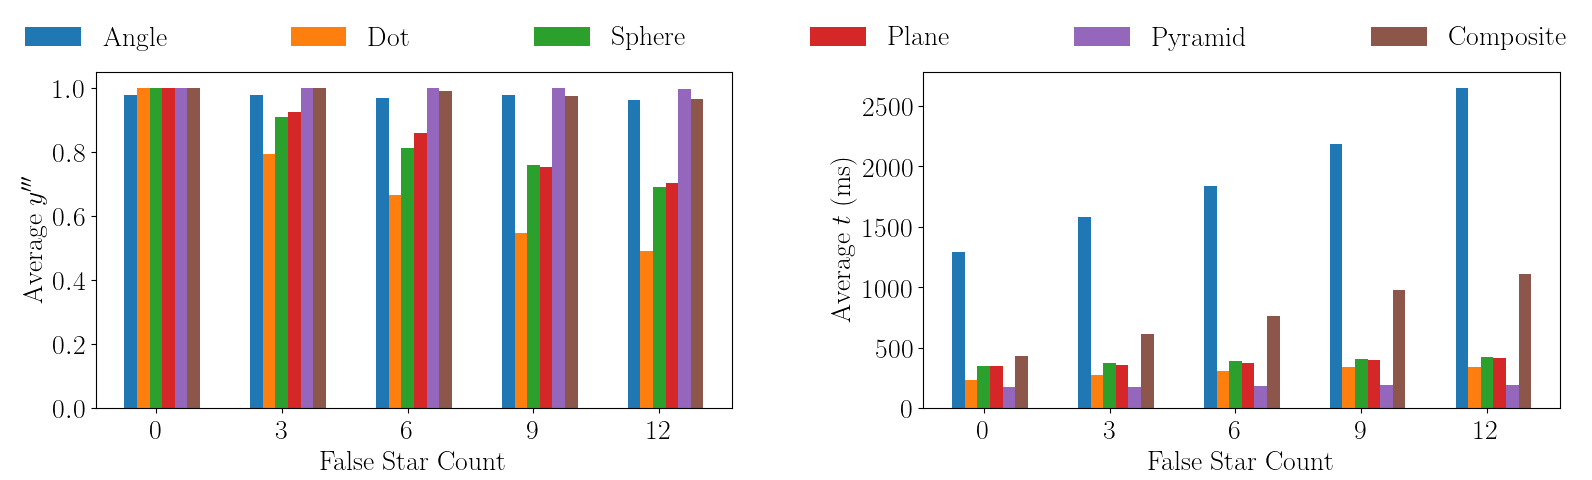
\includegraphics[scale=0.45]{images/identification-false-exp.png}
    \caption{
    Both plots depict the effect of varying the number of false stars on the average accuracy (left) and average running
    time to produce a map $a$ (right) for different identification methods.
    The field-of-view is bounded by $f = 20^\circ$ and the apparent magnitude is bounded by $m = 6.0$.
    Each method was capped at 500 query steps before erroring out and producing a false result.
    Each point represents the average of 1000 identification steps.
    } \label{figure:identificationFalse}
    }
\end{figure*}
